\documentclass[10pt,journal,compsoc, draftclsnofoot,onecolumn]{IEEEtran}

\usepackage{graphicx}

\title{
    Requirements
    \\3D object pose tracking for Robotics Grasping
    \\Lux Vision
    \\CS461 Fall 2017
}

\author{Connor Campbell, Chase McWhirt, Jiawei Mo}

\begin{document}
\maketitle

\begin{abstract}
As robots and artificial intelligence become increasingly important in the modern age, they will need to be able to interact with their environment on their own, and computer vision is an integral part of a robot's understanding of its surroundings.
Oregon State University's robotics department has an ongoing project attempting to improve computer vision, and this Capstone project is aimed at furthering that goal.
%Specifically, using machine learning to help a computer make appropriate adjustments to its calculations based on changes in lighting.
Specifically, this Capstone project will be the culmination of implementing various dynamic masking techniques that can be executed in real time.
\end{abstract}
\pagebreak


\tableofcontents
\pagebreak


\section{Purpose}
This document will define the goals given by the client.
The goals will include specific tasks that can be accomplished by a single person.
These tasks will be defined in such a way that they are easily distributed among the group members.
Tasks will also effectively be verifiable.


%\subsection{Scope}
%The software will be able to determine the lighting conditions in a given image, then use that information to determine what parts of the image include the object it's looking for. Taking lighting conditions into account will allow the computer to be more selective when identifying pixels as part of the object it's looking for, which will reduce the number of false positives without losing accuracy. This will improve the computer's ability to interact with the environment with a robot arm.


\section{Overview}

\subsection{Product Perspective}
%The object tracking system currently used by the University's robotics team has an issue with lighting. Shadows and different lighting intensities result in the objects the computer is looking for appearing as different colors. Currently, it accounts for this by identifying a large range of colors as potentially being part of the object. This, of course, results in a lot of false positives (pixels being labeled as part of the object when they actually aren't). This new approach will allow the computer to adjust the expected average for the specific lighting with a smaller acceptable range.

%If the new programs prove to be more accurate than the ones currently in use, then the old identification system will be swapped out for the new one. As such, the differences in how the program interacts with the rest of the project should be minimal, to ensure a smooth transition.
The project is only a piece of a much larger project.
The larger project is a robotic grasping problem.
Oregon State University has a robotic arm that should be able to grasp and manipulate an object within a specific environment.
The environment will be a box containing the desired object for manipulation, the robotic arm, a single light source, and two cameras placed on adjacent corners of the ceiling.
This particular robotic arm has no tactile sense.
Thus, it must be able to understand the entire environment with only optical input.
The project discussed in this document is geared to solving the problem of handling optical input.
The current code behind this functionality is able to understand its environment by finding cross sections within its two camera inputs.
This effectively gives the robot stereo vision.
However, its sense of objects is extremely limited.
The code behind the robotic arm attempts to create a mask over important objects in the scene.
This functionality expects uniform color though.
Since the environment only contains a single light source, it is essentially impossible for an important object to be uniformly colored.
Light diffusion will make an object appear covered in a wide variety of shades.
If there were multiple light sources, this effect could be decreased.
However, since an object is going to be manipulated, creating perfect lighting conditions is highly unrealistic.

\noindent
It should be noted that these functions will primarily be used by the University's robotics research team.
They won't be robust enough for complex, real world applications, but are rather meant to be a step forward for future research.


\subsection{Product Functions}
%The first function will determine the lighting diffuse and specular of the scene. It will be created using machine learning. In this case, the input will be an image (in the form of the color values of each pixel), and the outputs will be seven numbers that accurately describe the lighting of the scene.

%The second function will then use the information provided by the first to identify which pixels in the image belong to the object. The larger project already has a means of determining an approximate mask of the image, so our function will use that along with the lighting information to generate a more precise mask. This may also utilize machine learning.
In order to solve the problem of inconsistent light sources, this project will have to create and execute a more dynamic method of image masking to accurately identify the object.
The client has discussed multiple possible approaches to do this, but is not sure which method will work best.
There will be three different implementations attempted and these will be tested against a straw man implementation.
The best implementation measured against the straw man will become the final product.
This project will only attempt to find the best masking function for identifying the robotic arm itself.
As stretch goals, the best method found in the main project will be implemented to mask the object the robotic arm will grasp.
As a final stretch goal, both masking methods will be verified as compatible with each other.


%\subsubsection{User Characteristics}
%These functions will primarily be used by the University's robotics research team. They won't be robust enough for complex, real world applications, but are rather meant to be a step forward for future research.


\subsection{Constraints}
This phase is a part of a big project.
Our group is to undertake only the lighting changes during object grasping.
As such, it will need to interact appropriately with the rest of the project.
Since this program is meant to replace an older identification system, it will be ideal for the inputs and outputs to be similar, in order to minimize the need for adjustments to the rest of the project.


\section{System Requirements}

\subsection{Functional requirements}
%The end product will be two helper functions for the computer vision project.
%The first will take an image of a scene and the initial position of the object being tracked as input and determine the diffuse and specular that describe the lighting of the scene.
%These will be used to determine the color range that the computer should be looking for.
%The second function will then use the images, diffuse, specular, and the approximate mask in order to determine a more accurate final mask.
%The primary goal is to get these functions to properly track a robotic arm, and as a stretch goal is to attempt to do the same with a set of objects that the arm can manipulate.

%Both of these functions will be made with machine learning.
%They will be trained with a video of the arm moving around in such a way as to cast a shadow on itself, as well as in different lighting scenarios.
%About one hundred and fifty key frames will be taken from the video for training and testing data.
%The specular and diffuse will be measured by hand, as well as an accurate mask for the robotic arm using a image editing software, such as Photoshop.
%The functions will be fed this data for it to train itself, and when it's done, it will be tested for accuracy.
To begin, this project will be based on images and pose transforms that our client has gathered.
These images will be of the robotic arm in various poses, and will be used both for training and testing the algorithms.
The initial straw man will be determined by simply running a k-means clustering over all of the data to determine a color range to look for.
Next, the images will be grouped based on the arm’s pose.
Each group will have its own version of each of the three methods.
The three methods include another k-means clustering (though over a single group as opposed to all of the data), neural networks, and support vector machines.
The method that 



\subsection{Performance requirements}
%There are two primary performance requirements that we will be aiming for.
%The first is for the final mask to label at least 95\% of the pixels in a given image correctly, as opposed to the 80\% accuracy of the method currently being used.
%The second requirement is to reduce the size of the color range the computer is looking for.
%The current method attempts to make up for variations in lighting and shade by using a large range of acceptable colors to be identified as the object.
%Since the new method can account for the lighting on its own and adjust the expected average accordingly, we hope to reduce the range by a factor of ten, reducing the number of false positives, without losing a significant amount of true positives.
The goal is for the best of the three methods to replace part of the larger project’s current system.
As such, it should label at least 80\% of the pixels correctly as either part of the arm or not.
Ideally, it should have at least 90\% accuracy, but 80\% will at least be an improvement.


\section {Verification}
% The accuracy of the functions is rather simple to verify.
% All need be done is for some of the example problems to be saved for testing purposes.
% Provide the inputs for the examples to the functions and compare the output to the expected output.
% If a function answers some examples with sufficiently low accuracy, new examples similar to the ones it failed on can be generated specifically to train it for those scenarios.
Implementation effectiveness can be measured in two distinct ways.
First, it can be measured against a designated "truth" defined when images were manually masked.
Each pixel will fall into four groups.
True positives will be a particular implementation masking a pixel as part of the robot arm being correct.
True negatives will be masking a pixel as not part of the arm and being correct.
False positive will be masking a pixel as part of the arm and being incorrect.
Finally, false negative will be masking a pixel as part of the arm and being incorrect.
The client has established that false negatives are worse than false positives.
This is because false positives could exist due to environmental conditions such as background color.
False negatives mean that the algorithm has failed to correctly identify the arm through flaws in implementation or even the algorithm itself.
The client has also stated a desired accuracy of 80\% or more, though, she has also said this is not a hard requirement.
Rather, 80\% is an arbitrary amount she expects will be practically effective, though the percentage could be lower or higher.

\noindent
The other way to verify each implementation is whether or not it is more effective than the straw man.
If it is less effective, the implementation fails.
If it is more effective, it passes.
It is possible to measure how much more effective the implementation is over the straw man.
For example, if the straw man has 40\% of all true positives and implementation x has 80\% of all true positives, implementation x is twice as effective at defining true positives than the straw man.
This concept will be important for defining how successful any implementation is.


\newpage
\section{Definitions}
\begin{itemize}
\item K-means Clustering - An algorithm that involves dividing a group of data points into smaller groups such that each point is in the group with the group average most similar to it.

\item Mask - An overlay defining a set of pixels as a unique object.
Applying a mask over an object is the main goal of the project.

\item Neural Network - A form of machine learning designed to mimic the activity of organic brains by simulating neurons firing in order. This can be simplified as a multiplying a series of matrices to the input.

\item Stereo Vision - Also known as binocular vision, this is the mechanic of taking two images taken from different angles and defining a perceived depth.

\item Straw Man - In this instance, a straw man is an implementation that is expected to under perform.
An extreme general approach is tested and measured.
It then acts as a baseline metric to compare to other implementations.

%\item Support Vector Machine - ???

\end{itemize}

\section{Gantt Chart}
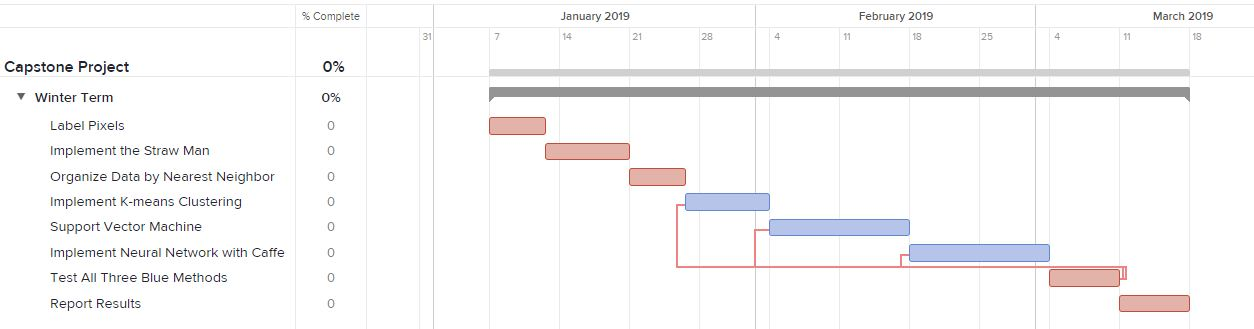
\includegraphics[width=\textwidth]{gantt_chart.JPG}

\end{document}